
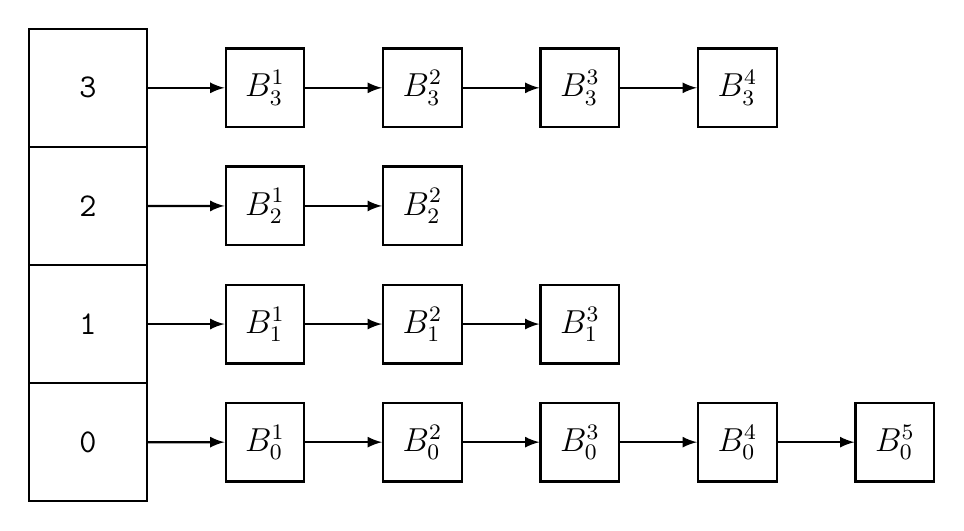
\begin{tikzpicture}[font={\fontsize{12pt}{12}\selectfont}]

    \node[rectangle, draw, color=black, thick, anchor=south west, minimum width=1.5cm, minimum height=1.5cm, inner sep=0pt] (c3) at (0, 4.5)    {\ttfamily 3};
    \node[rectangle, draw, color=black, thick, anchor=south west, minimum width=1.5cm, minimum height=1.5cm, inner sep=0pt] (c2) at (0, 3)      {\ttfamily 2};
    \node[rectangle, draw, color=black, thick, anchor=south west, minimum width=1.5cm, minimum height=1.5cm, inner sep=0pt] (c1) at (0, 1.5)    {\ttfamily 1};
    \node[rectangle, draw, color=black, thick, anchor=south west, minimum width=1.5cm, minimum height=1.5cm, inner sep=0pt] (c0) at (0, 0)      {\ttfamily 0};
   
    % C0 
    \node[rectangle, draw, color=black, thick, anchor=south west, minimum width=1cm, minimum height=1cm, inner sep=0pt] (b01) at (2.5, 0.25) {$B_0^1$};
    \node[rectangle, draw, color=black, thick, anchor=south west, minimum width=1cm, minimum height=1cm, inner sep=0pt] (b02) at (4.5, 0.25) {$B_0^2$};
    \node[rectangle, draw, color=black, thick, anchor=south west, minimum width=1cm, minimum height=1cm, inner sep=0pt] (b03) at (6.5, 0.25) {$B_0^3$};
    \node[rectangle, draw, color=black, thick, anchor=south west, minimum width=1cm, minimum height=1cm, inner sep=0pt] (b04) at (8.5, 0.25) {$B_0^4$};
    \node[rectangle, draw, color=black, thick, anchor=south west, minimum width=1cm, minimum height=1cm, inner sep=0pt] (b05) at (10.5, 0.25) {$B_0^5$};
    \draw[-latex, thick] (c0) -- (b01);
    \draw[-latex, thick] (b01) -- (b02);
    \draw[-latex, thick] (b02) -- (b03);
    \draw[-latex, thick] (b03) -- (b04);
    \draw[-latex, thick] (b04) -- (b05);

    % C1 
    \node[rectangle, draw, color=black, thick, anchor=south west, minimum width=1cm, minimum height=1cm, inner sep=0pt] (b11) at (2.5, 1.75) {$B_1^1$};
    \node[rectangle, draw, color=black, thick, anchor=south west, minimum width=1cm, minimum height=1cm, inner sep=0pt] (b12) at (4.5, 1.75) {$B_1^2$};
    \node[rectangle, draw, color=black, thick, anchor=south west, minimum width=1cm, minimum height=1cm, inner sep=0pt] (b13) at (6.5, 1.75) {$B_1^3$};
    \draw[-latex, thick] (c1) -- (b11);
    \draw[-latex, thick] (b11) -- (b12);
    \draw[-latex, thick] (b12) -- (b13);

    % C2 
    \node[rectangle, draw, color=black, thick, anchor=south west, minimum width=1cm, minimum height=1cm, inner sep=0pt] (b21) at (2.5, 3.25) {$B_2^1$};
    \node[rectangle, draw, color=black, thick, anchor=south west, minimum width=1cm, minimum height=1cm, inner sep=0pt] (b22) at (4.5, 3.25) {$B_2^2$};
    \draw[-latex, thick] (c2) -- (b21);
    \draw[-latex, thick] (b21) -- (b22);

    % C3 
    \node[rectangle, draw, color=black, thick, anchor=south west, minimum width=1cm, minimum height=1cm, inner sep=0pt] (b31) at (2.5, 4.75) {$B_3^1$};
    \node[rectangle, draw, color=black, thick, anchor=south west, minimum width=1cm, minimum height=1cm, inner sep=0pt] (b32) at (4.5, 4.75) {$B_3^2$};
    \node[rectangle, draw, color=black, thick, anchor=south west, minimum width=1cm, minimum height=1cm, inner sep=0pt] (b33) at (6.5, 4.75) {$B_3^3$};
    \node[rectangle, draw, color=black, thick, anchor=south west, minimum width=1cm, minimum height=1cm, inner sep=0pt] (b34) at (8.5, 4.75) {$B_3^4$};
    \draw[-latex, thick] (c3) -- (b31);
    \draw[-latex, thick] (b31) -- (b32);
    \draw[-latex, thick] (b32) -- (b33);
    \draw[-latex, thick] (b33) -- (b34);

    %\draw[latex-, thick] (c0.west) -- (-0.5, 0.75);

\end{tikzpicture}
